\chapter{Discussion} % Main chapter title

\label{Chapter5} % Change X to a consecutive number; for referencing this chapter elsewhere, use \ref{ChapterX}


%----------------------------------------------------------------------------------------
%	SECTION 1
%----------------------------------------------------------------------------------------
When an HMD is deployed, users struggle to understand their surroundings, identify their orientation and determine where they are in relation to other objects such as walls and users in their physical space. 
In consideration of this, it is highly likely that users wearing HMDs collide with other users and walls. 

To resolve this problem, the proposed method employs a strategy with a time-dependent synced-rotational gain to avoid collisions between multiple VR users sharing the same physical space. The results mentioned in the previous chapter prove that the proposed method works better than the Holm's one. This chapter describes some concerns that would affect the results. 
\section{Motion sickness}
From Fig.~\ref{fig:SSQ_CtoS_Of_RorationEx} to Fig.~\ref{fig:SSQ_Acc_Of_RotationEx} on rotation awareness experiments, the subjects manifested symptoms at slight and moderate levels and they could continue the experiments.
From Fig.~\ref{fig:SSQ_ConstantOfCurvatureEx} and Fig.~\ref{fig:SSQ_AccOfCurvatureEx} on curvature distance experiments, two subjects from five subjects manifested symptoms in severe level. During the experiment on curvature distance, two of the five subjects started to have eye strain and difficulty in focusing the given task at the speed of rotation of 3.2deg/s. However, they said they could overcome motion sickness if they could take a break and then I temporarily suspended them for the extra rest time of five minutes. While they had a rest time, I recommended them to see the outside of the room such as trees and the nearby buildings. After that, their motion sickness had been reduced to a low level and they continued the task and did not experience motion sickness.

\begin{figure}[H]\centering
	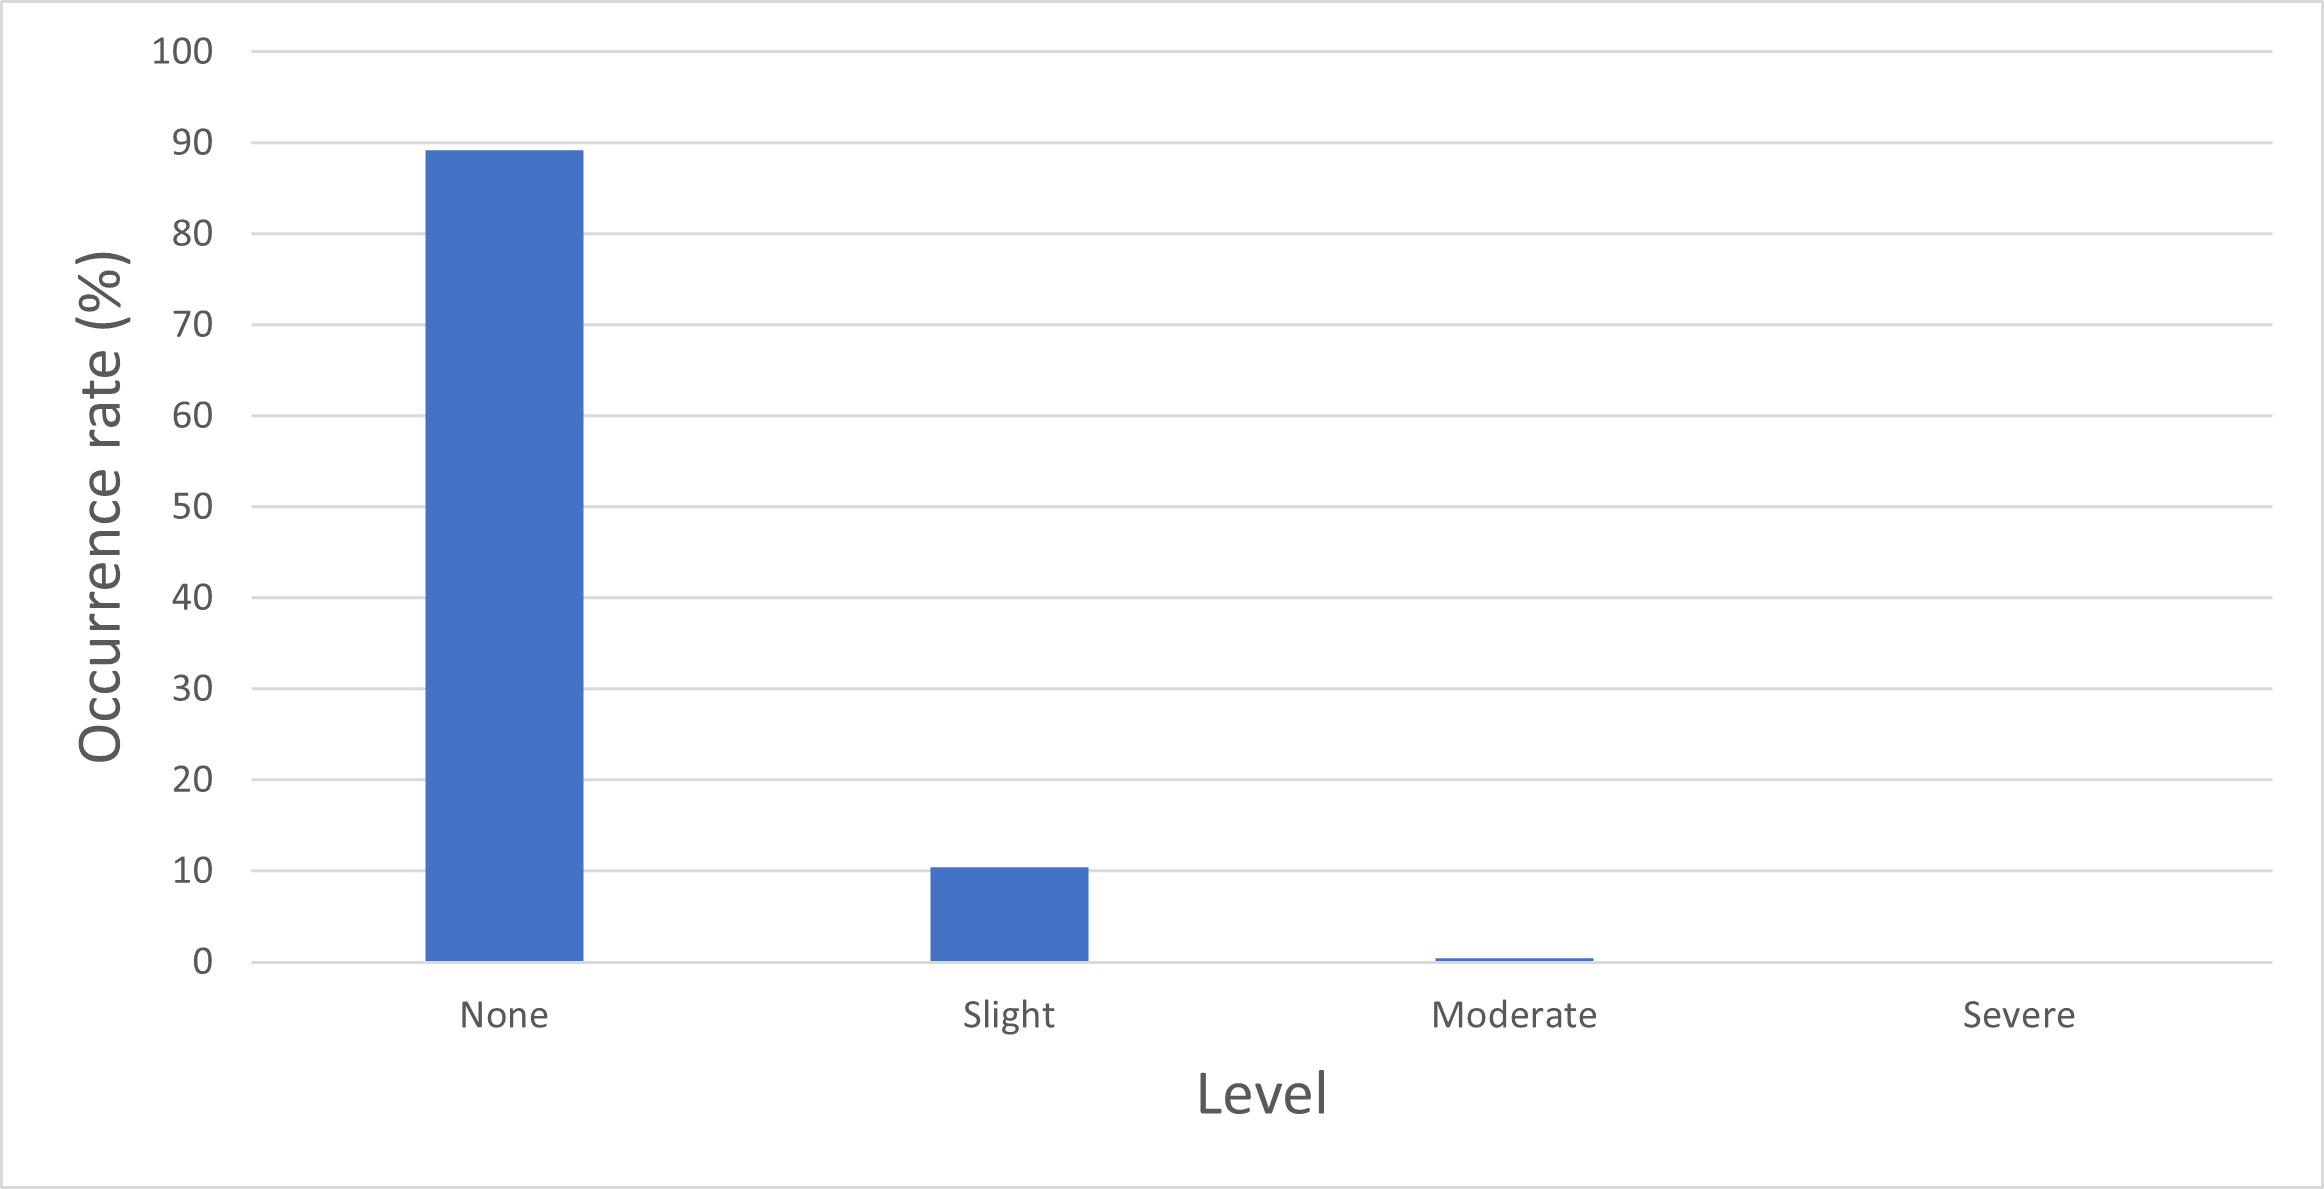
\includegraphics[width=0.9\textwidth]{Pictures/SSQ_StoC_Of_RorationEx.png}%imagine location
	\caption{SSQ results for the stop to constant speed rotation task.}\label{fig:SSQ_StoC_Of_RorationEx}%use name for ref.
	
\end{figure}
\begin{figure}[H]\centering
	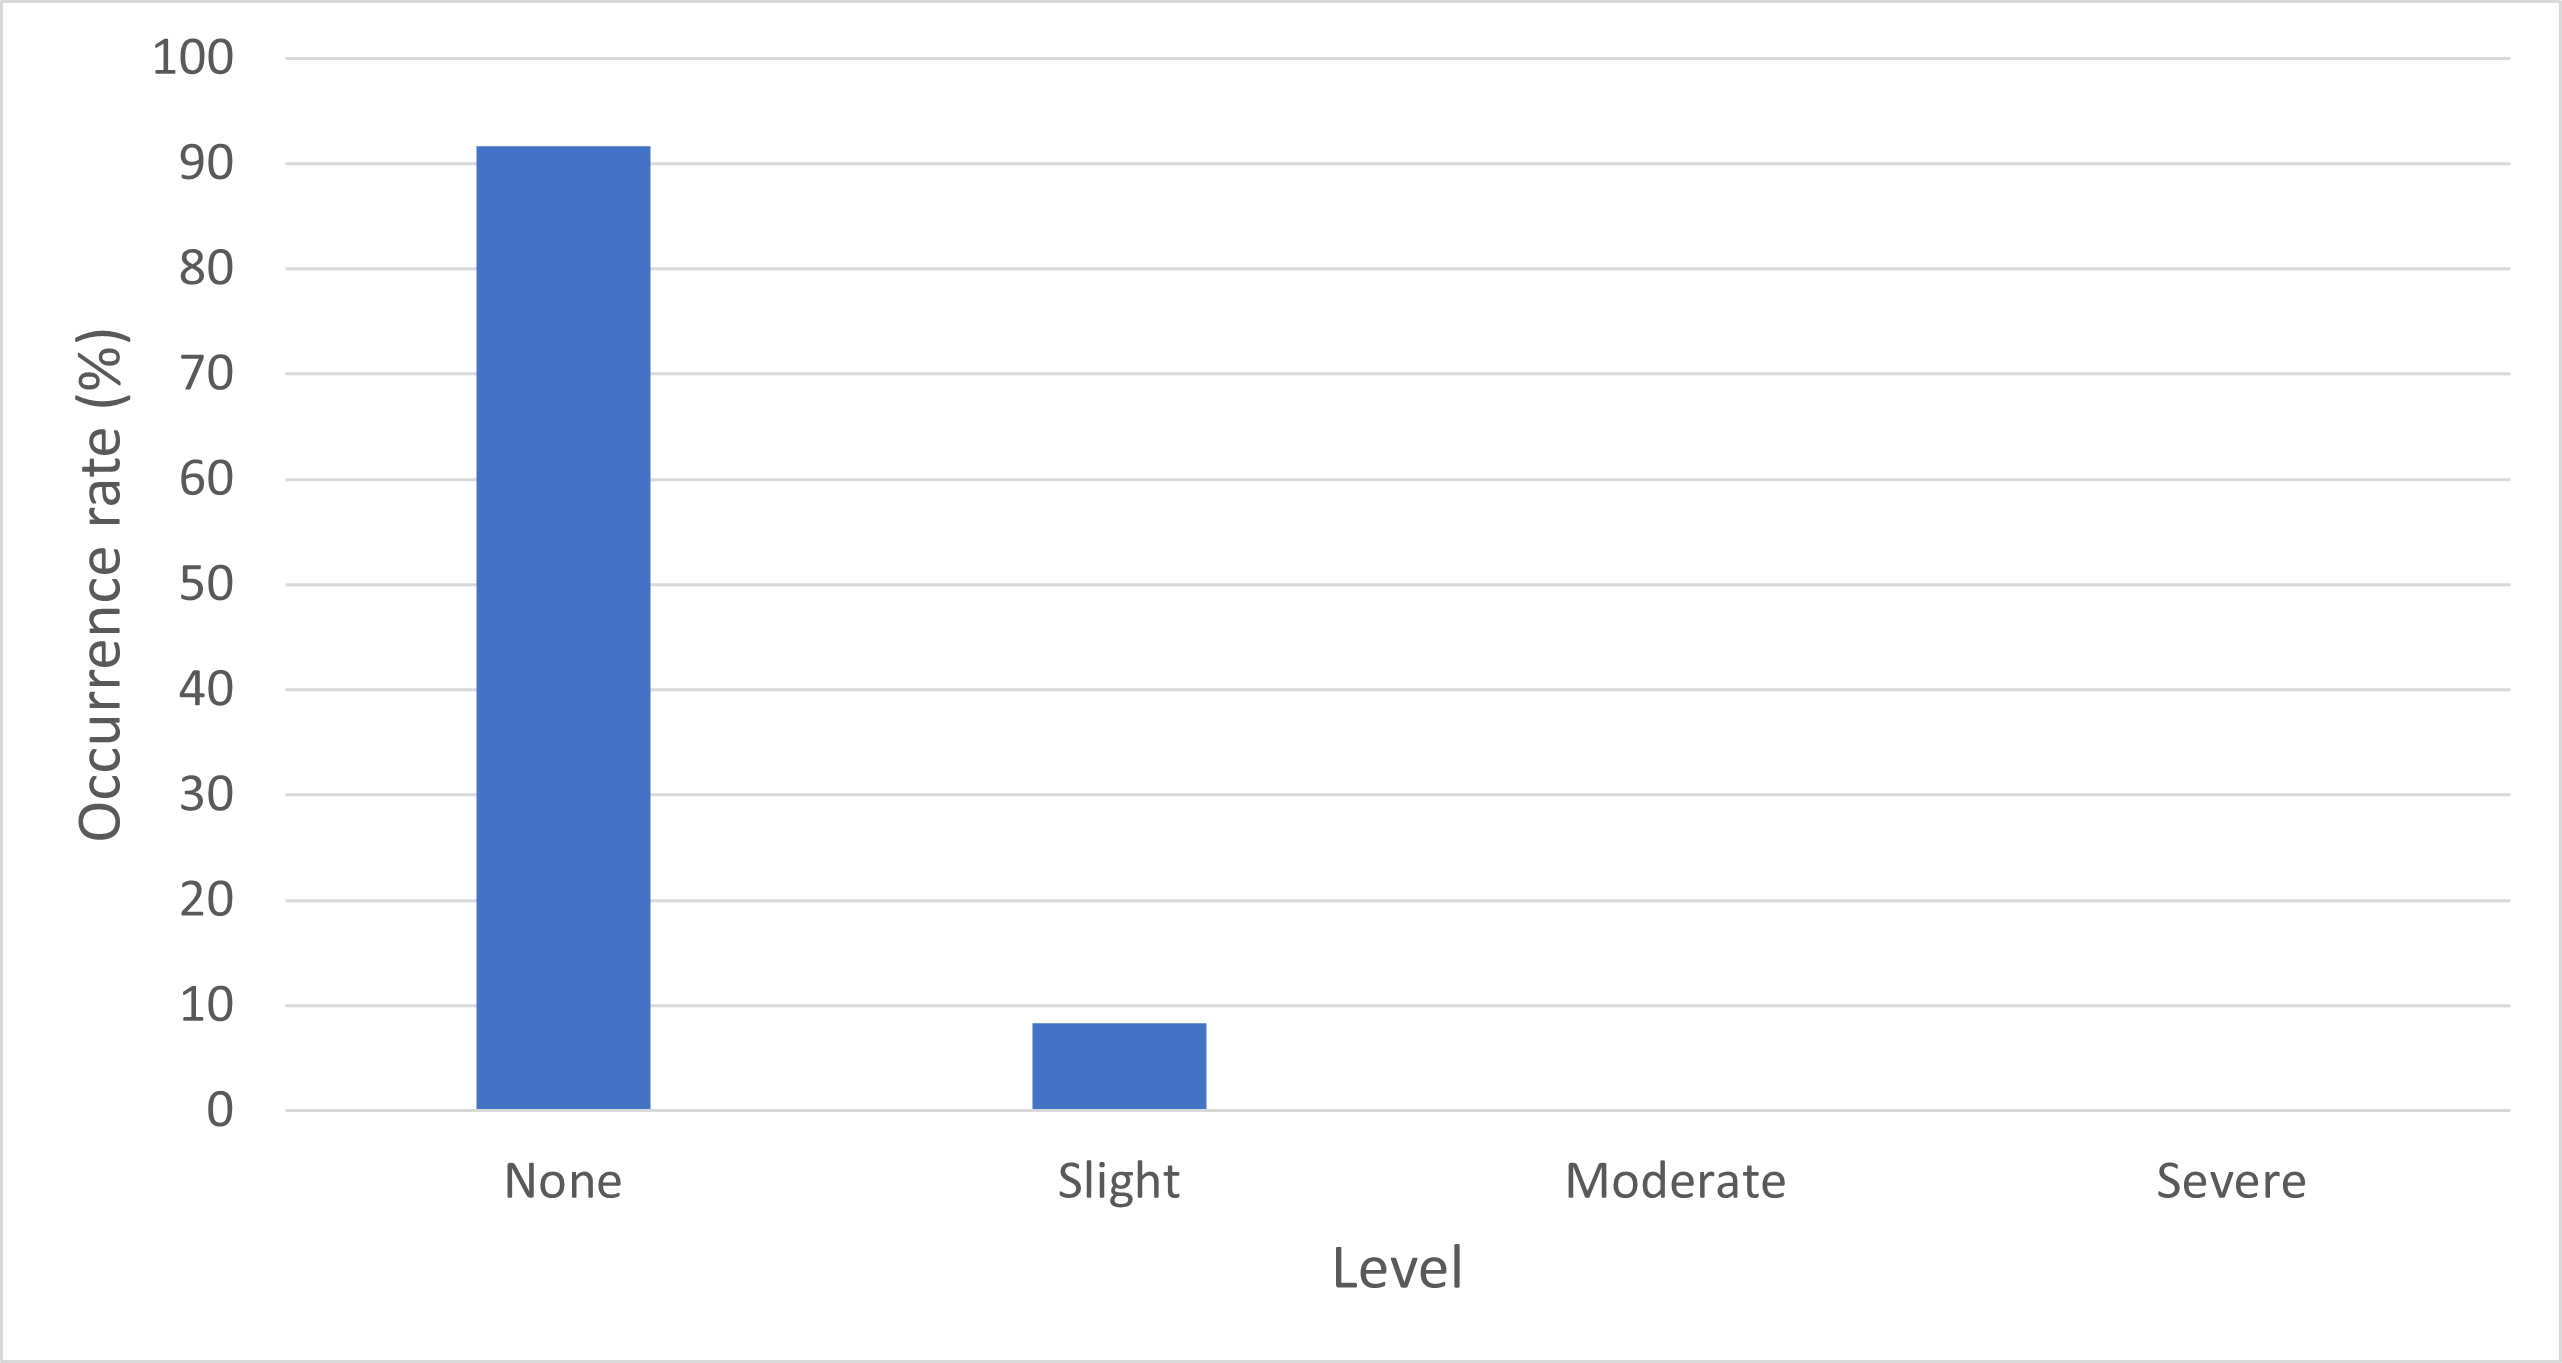
\includegraphics[width=0.9\textwidth]{Pictures/SSQ_CtoS_Of_RorationEx.png}%imagine location
	\caption{SSQ results for the constant speed to stop rotation task.}\label{fig:SSQ_CtoS_Of_RorationEx}%use name for ref.
	
\end{figure}
\begin{figure}[H]\centering
	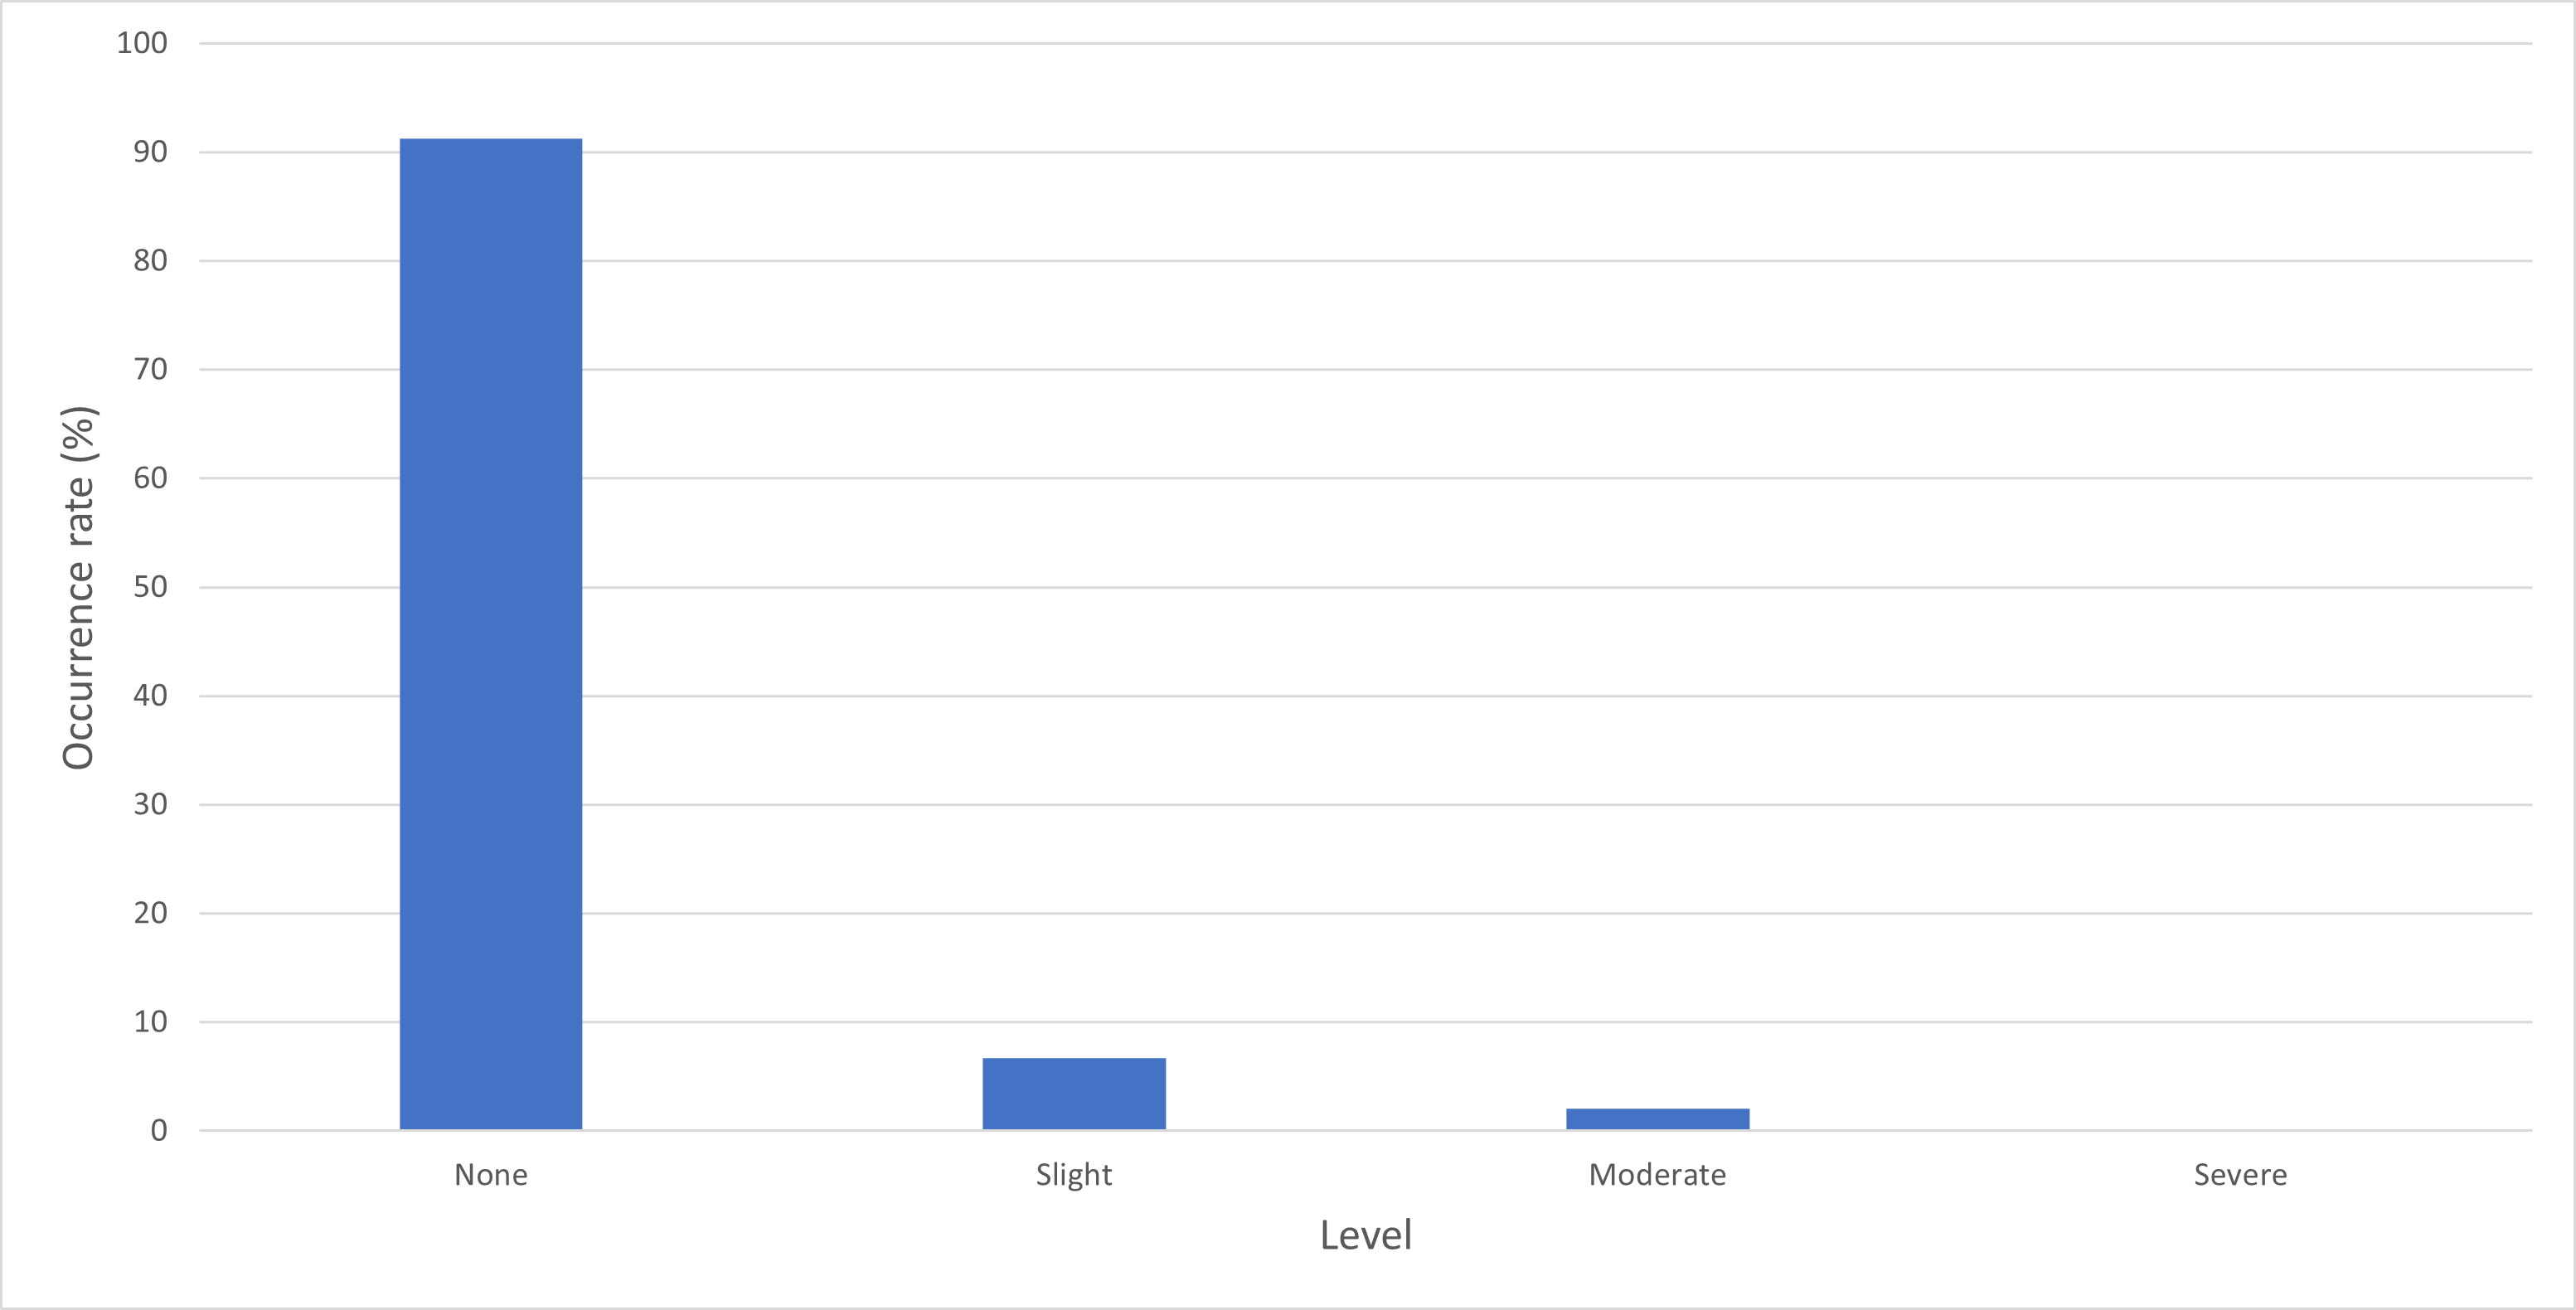
\includegraphics[width=0.9\textwidth]{Pictures/SSQ_Dec_Of_RotationEx.png}%imagine location
	\caption{SSQ results for the deceleration rotation task.}\label{fig:SSQ_Dec_Of_RotationEx}%use name for ref.
	
\end{figure}
\begin{figure}[H]\centering
	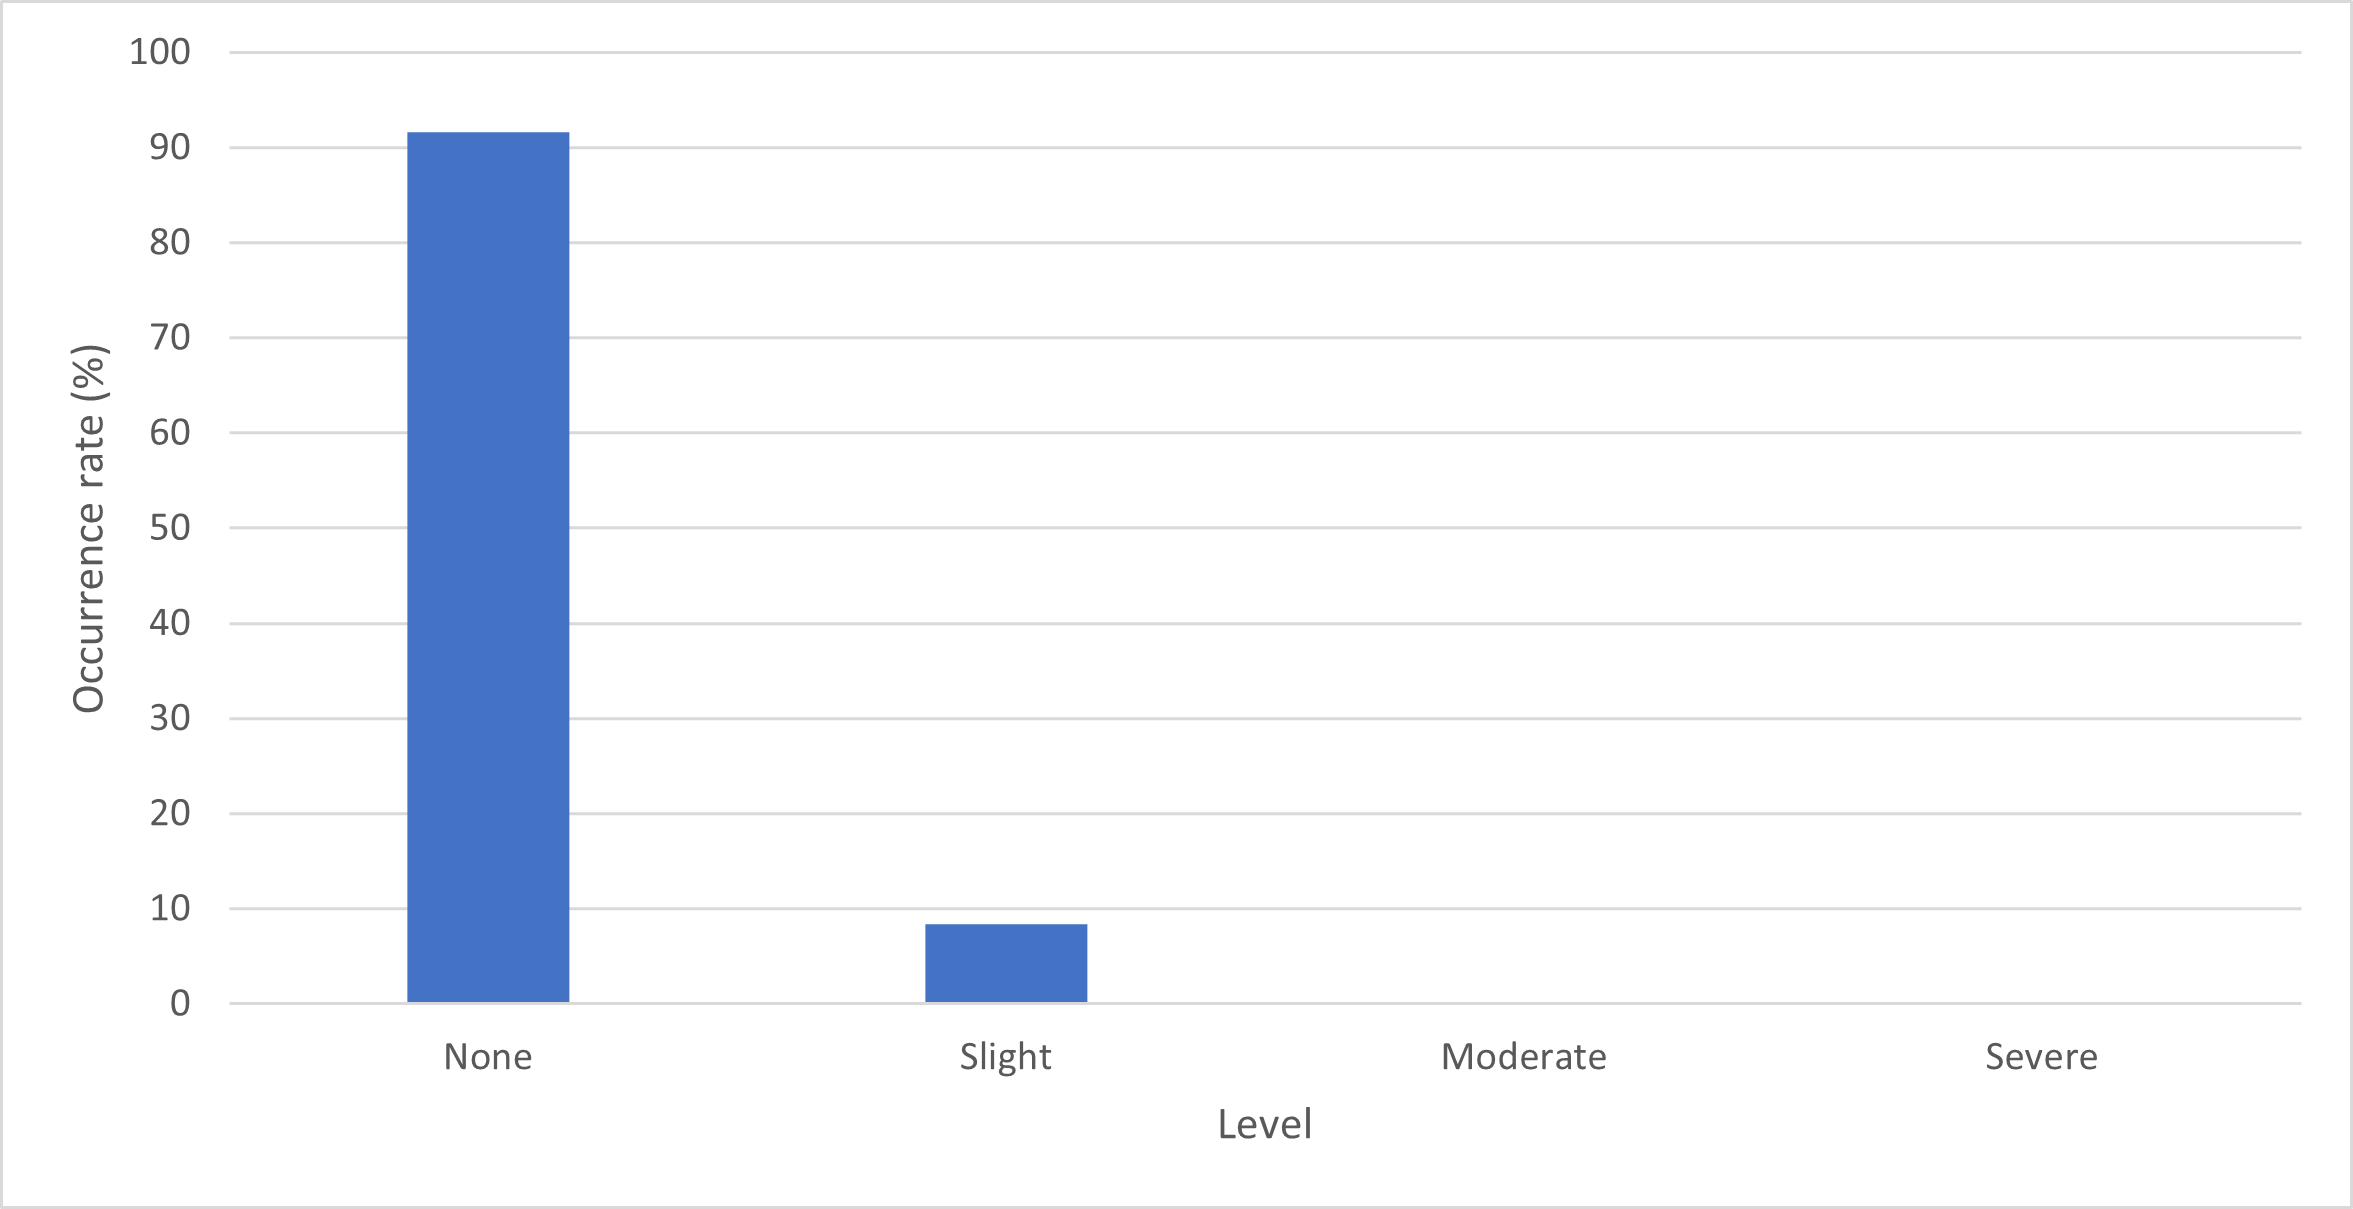
\includegraphics[width=0.9\textwidth]{Pictures/SSQ_Acc_Of_RotationEx.png}%imagine location
	\caption{SSQ results for the acceleration rotation task.}\label{fig:SSQ_Acc_Of_RotationEx}%use name for ref.

\end{figure}
\begin{figure}[H]\centering
	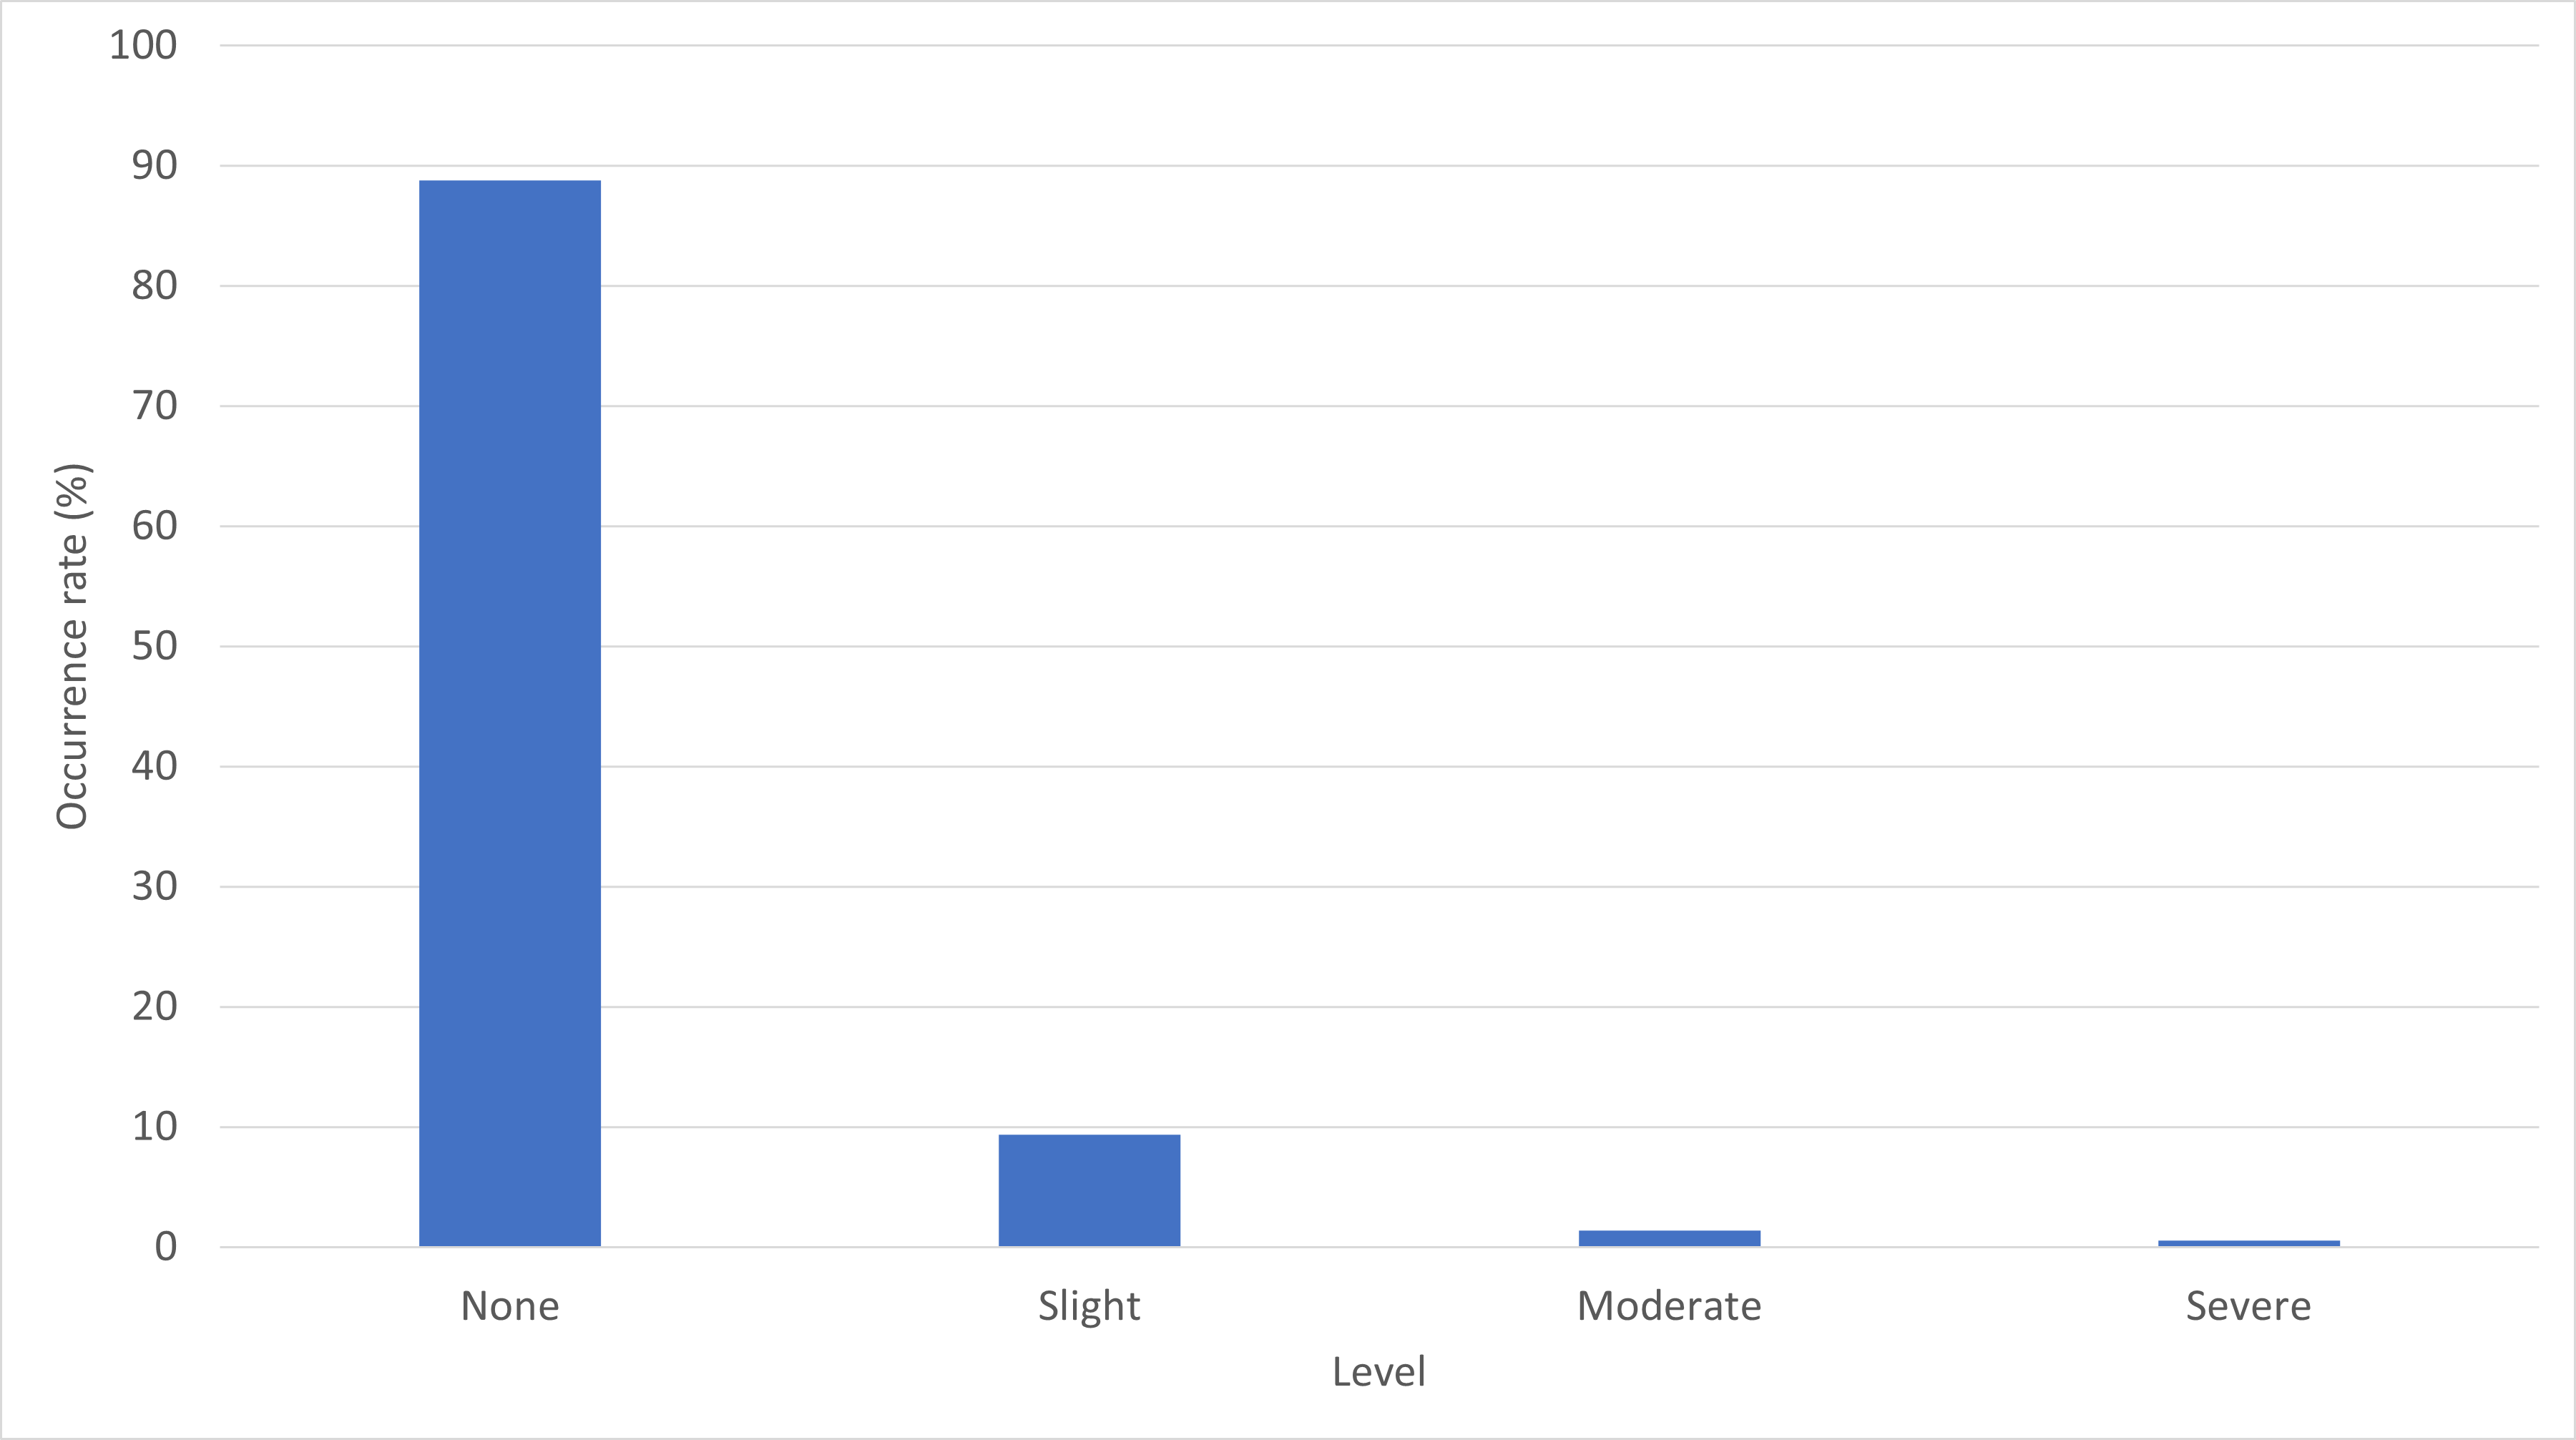
\includegraphics[width=0.9\textwidth]{Pictures/SSQ_ConstantOfCurvatureEx.png}%imagine location
	\caption{SSQ results for the constant speed task.}\label{fig:SSQ_ConstantOfCurvatureEx}%use name for ref.
	
\end{figure}
\begin{figure}[H]\centering
	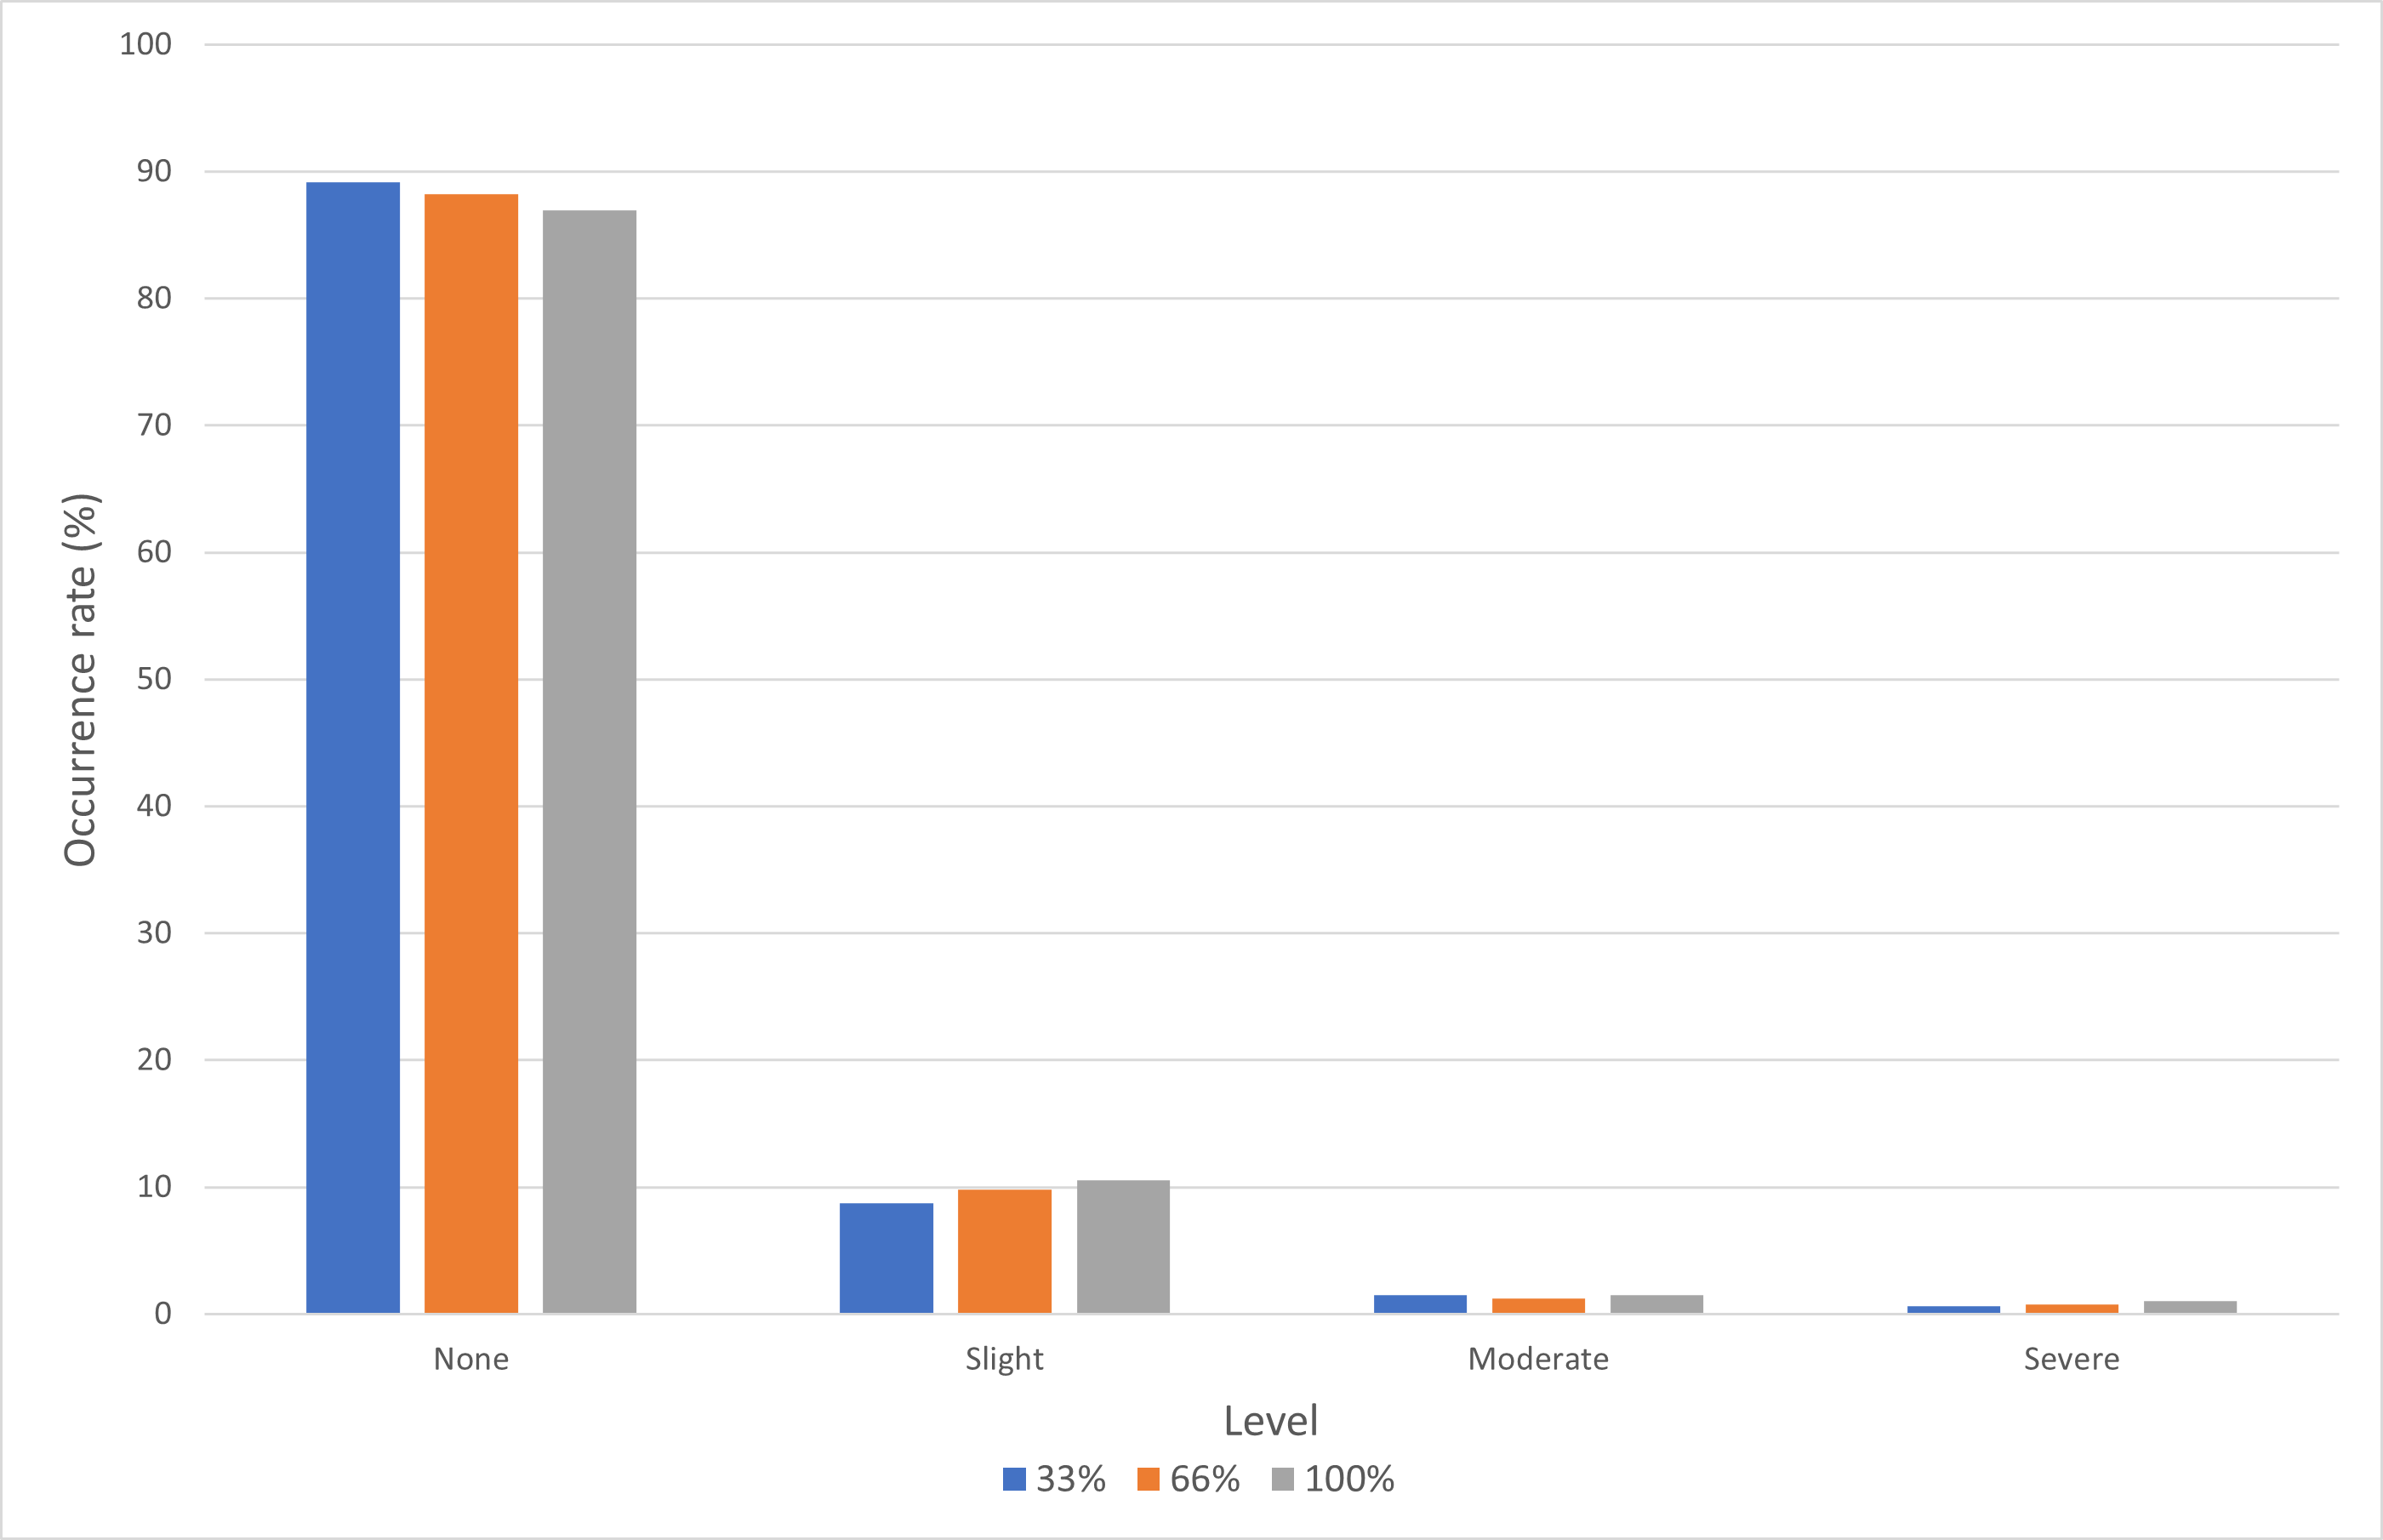
\includegraphics[width=0.9\textwidth]{Pictures/SSQ_AccOfCurvatureEx.png}%imagine location
	\caption{SSQ results for the acceleration task.}\label{fig:SSQ_AccOfCurvatureEx}%use name for ref.
	
\end{figure}
\section{Deployment in the real scenario}
From the simulation result, collisions can be avoided efficiently by the proposed method. However, when the proposed method is applied to the real scenario, there should be room for discussion. The simulation of the proposed method has a restricted condition that is the speed of walking 0.5m/s. If it is more or less than 0.5 m/s, the collision avoidance would be possible to fail and the collision possibility would be high. The further experiment on the relation between the speed of walking, the speed of rotation, and curvature distance, are needed. 
\section{Shapes of physical spaces}
The proposed method was evaluated by simulation where the physical space was a rectangular room. Three sizes of physical spaces were taken into consideration: Large, Medium and Small. In the real scenario, there must be tables, bookshelves, sofas, etc. in a room, leading to a complicated walking space. It has an effect on the collision possibility. A further experiment on the relation between practical layouts of a room and performance of collision avoidance is needed. 
\section{Effect of simulation frame rate on collision prediction}
The simulation ran on the Unity engine in the experiment. In Unity, to advance the simulation each step, Update() function is called to change properties of objects before they are rendered at each frame. The interval between Update() calls varies depending on an amount of rendering loads. If the interval slowed down, the collision prediction would not work properly. Because each agent walks at the speed of 0.5m/s, the distance he/she travels between frames is 0.83cm when the frame rate is 60 frames per second or fps. Fig.~\ref{fig:framerate} shows the relation between frame rates and the number of agents. The lowest frame rate is 51.13629 and the distance each agent travels between frames is 0.978cm in that case. This frame rate is expected not to affect the collision prediction.
%For testing the first experiment, we had a subject (5 people) and gave them to wear and try to notice the rotation in the virtual environment. We discussed and recorded the time for subjects to notice the rotation speed of (0.4deg/s, 0.8deg/s, 1.6deg/s, 3.2deg/s, 6.4deg/s and 12.8deg/s) when stop to constant speed and constant speed to stop rotation. In additional, we recorded the time for subjects to notice the deceleration and acceleration of (33\%, 66\% and 100\%) and the max rotation speeds are 0.4deg/s, 0.8deg/s, 1.6deg/s and 3.2deg/s. We knew the notice time of users, but we did not know about the rerated of a virtual environment and physical space distance in user moving situations. Also, while the user is walking the scene that we created in the program and we need them to rotate to make the curvature distance to avoid a collision with other users. We had to consider the average of half the width of a human shoulder (23cm) that affects the user's moving to avoid a collision with other users. So, we did another experiment that let the subject walk in a virtual environment and measured the distances in the constant speed task and acceleration task.
%From the result of both experiments, we had enough of the actual situation's information to make the simulation for multiple users (2 to 15). Based on the previous experiments' data, we create the simulation that the colliding users will be rotated while walking to avoid the collision when the collision is detected. When more than two users collide, all of the colliding users will be rotated. From the discussion, we need to know the proposed method's efficiency, and then we find the other method for comparing. We found that Holm's method is often used to avoid collisions between users. Then, we create Holm's method simulation. As more than two users share a physical place, we concluded that the proposed method is better compared to Holm's way because when three or more users have predicted a collision at the same time, Holm's method can be enabled collision avoidance function for only even number of users. When the number of users becomes an odd number, Holm's method can not notice some users and fail to collision avoidance, but the proposed method can enable a collision avoidance function that can be predicted for a collision of multiple users. Also, the proposed method's count of collision is lower than Holm's method and the count of successful avoidance is higher than Holm's method.
\begin{figure}[H]\centering
	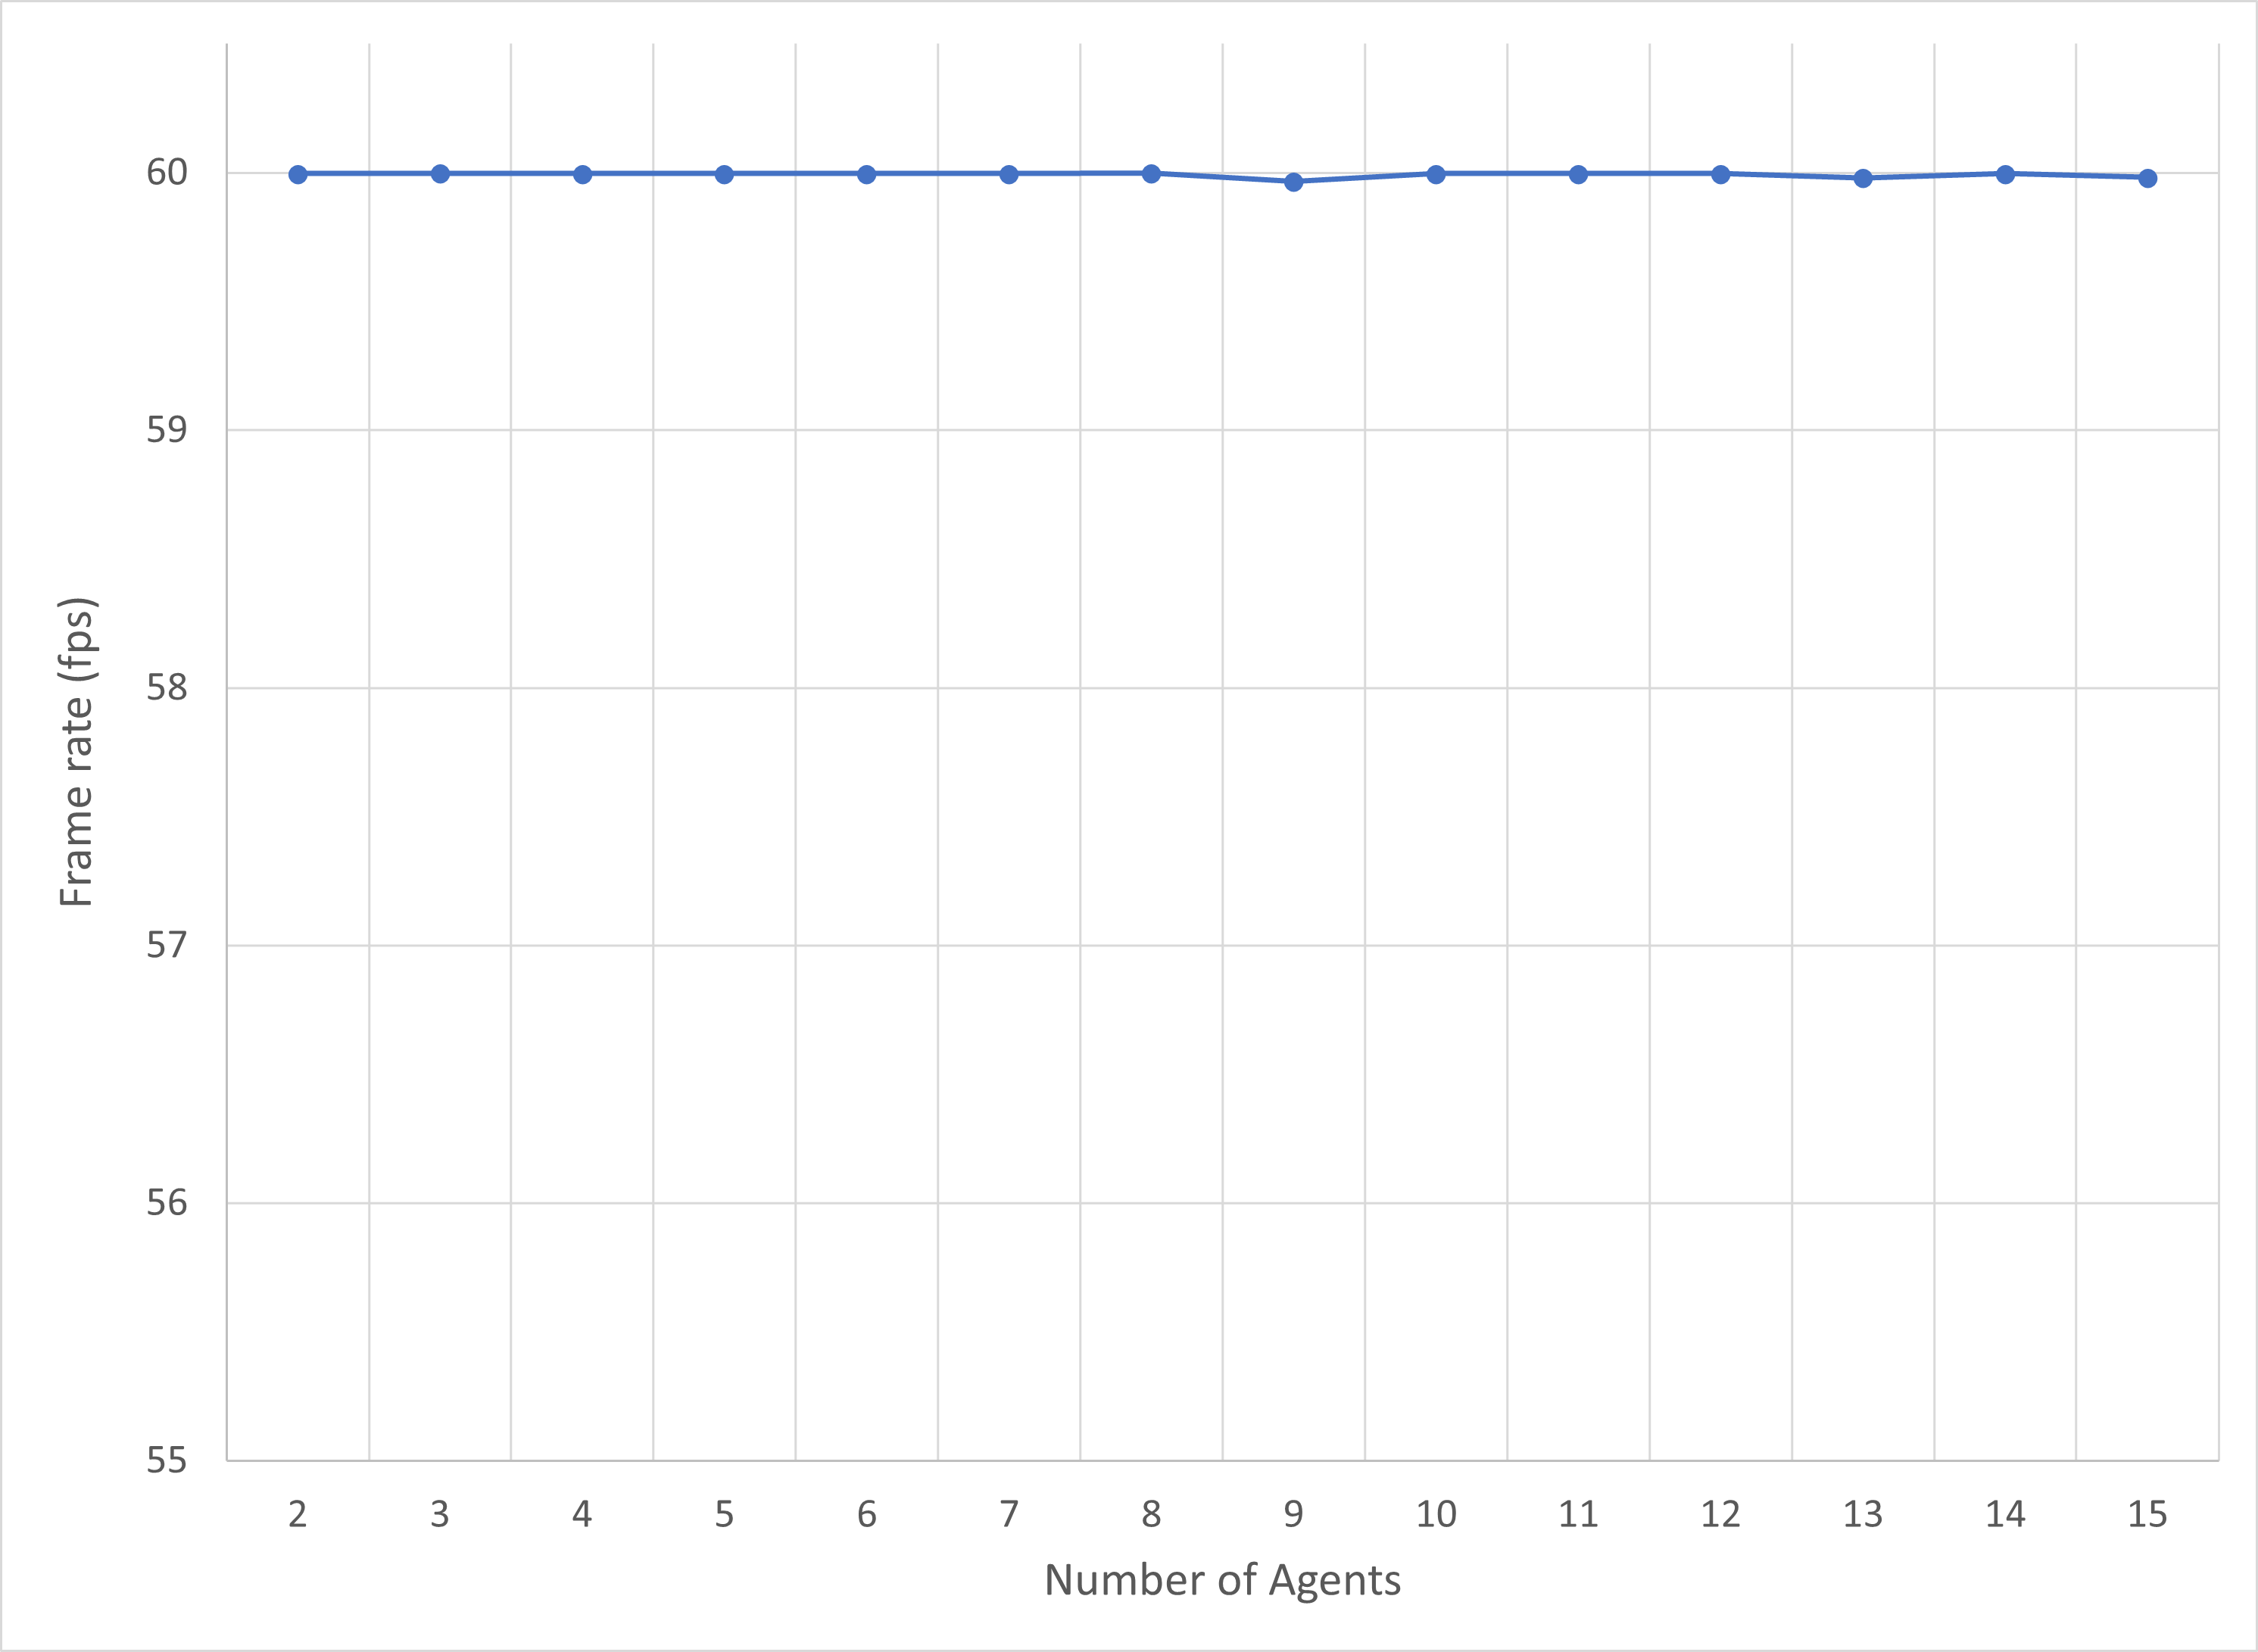
\includegraphics[width=1.0\textwidth]{Pictures/framerate.png}%imagine location
	\caption{Average of frame rate at each the number of agents.}\label{fig:framerate}%use name for ref.
	
\end{figure}